\chapter{Transmission Losses and AC Validation}

The lossless model ignores the power dissipated in the lines. This chapter adds losses to the dispatch and checks every dispatch with a full AC load flow, which also reveals the voltages and line loadings that ELD does not model.

\section{Loss formula from the network}
The B-coefficients are derived from the line data rather than taken as given. With bus 1 as the slack, the DC power-transfer distribution factors (PTDF) give the line flows $f = \mathrm{PTDF}\,(C_g P - P_d)$ in per unit, where $C_g$ places each generator at its bus. With voltages close to 1~pu, the losses are $\sum_\ell r_\ell f_\ell^2$. Expanding this square gives Kron's loss formula \cite{wood2014}
\begin{equation}
\PL = P^\top B P + B_0^\top P + B_{00},
\end{equation}
where $B$, $B_0$ and $B_{00}$ depend on the line resistances, the PTDF and the bus loads of the period. The loss-inclusive balance is $\sum_i P_i = \PD + \PL(P)$.

\section{Newton--Raphson AC load flow}
A polar Newton--Raphson load flow with the analytic Jacobian of MATPOWER \cite{matpower2011} was written for the network (lines modelled as $\pi$ sections; bus 1 slack at 1.05~pu; buses 2 and 3 PV at 1.05 and 1.07~pu; loads at power factor 0.98). It was validated against PYPOWER on MATPOWER \texttt{case6ww}: the slack output (107.875~MW), total losses (7.875~MW), generator reactive powers (15.96, 74.36 and 89.63~MVAr) and all bus voltages and angles agree exactly. In this study the load flow converged in 4 iterations in every case.

\section{Hybrid QAOA with losses}
Because the QUBO must be quadratic, the loss term cannot be inserted directly into \eqref{eq:qubo}. An outer iteration is used instead:
\begin{enumerate}
\item Solve the QUBO with QAOA ($p = 3$) for demand $\PD + \PL^{(k)}$, starting with $\PL^{(0)} = 0$.
\item Refine the five best samples with SLSQP subject to the loss-inclusive balance, inside the $\pm1$-step box.
\item Update $\PL^{(k+1)} = \PL(P^{(k)})$ and repeat until the dispatch no longer changes.
\end{enumerate}
The iteration converged in 2 rounds in eleven periods and 3 in period 3.

\section{Results}
\begin{table}[H]
\centering
\caption{Dispatch with losses: costs, losses and AC load-flow checks for the hybrid QAOA dispatch.}
\label{tab:losses}
\small
\begin{tabular}{crrrrrcc}
\toprule
Period & SLSQP & Hybrid & Gap & $\PL$ formula & $\PL$ AC & $V_{\min}$ & T09 loading\\
 & (\$/h) & (\$/h) & (\%) & (MW) & (MW) & (pu) & (\%)\\
\midrule
1 & 3594.48 & 3594.48 & 0.000 & 5.34 & 5.12 & 1.021 & 108\\
2 & 3091.24 & 3091.24 & 0.000 & 3.76 & 3.61 & 1.027 & 89\\
3 & 2846.00 & 2848.25 & 0.079 & 3.12 & 3.05 & 1.030 & 73\\
4 & 2725.09 & 2725.09 & 0.000 & 2.74 & 2.66 & 1.032 & 74\\
5 & 2968.14 & 2968.14 & 0.000 & 3.41 & 3.27 & 1.029 & 84\\
6 & 3341.28 & 3342.01 & 0.022 & 4.59 & 4.41 & 1.024 & 96\\
7 & 3850.57 & 3850.88 & 0.008 & 6.17 & 5.95 & 1.018 & 118\\
8 & 4371.61 & 4371.61 & 0.000 & 8.12 & 7.94 & 1.012 & 134\\
9 & 4636.41 & 4637.13 & 0.016 & 9.17 & 9.03 & 1.009 & 145\\
10 & 4503.80 & 4503.82 & 0.000 & 8.65 & 8.49 & 1.011 & 138\\
11 & 4240.21 & 4240.21 & 0.000 & 7.61 & 7.41 & 1.014 & 130\\
12 & 3850.57 & 3850.88 & 0.008 & 6.17 & 5.95 & 1.018 & 118\\
\midrule
Total & 44019.39 & 44023.73 & 0.010 & 68.83 & 66.90 & & \\
\bottomrule
\end{tabular}
\end{table}

\subsection{Effect of losses on cost}
Losses of 2.7--9.2~MW raise the optimal cost by 1.2--2.6\,\% per period, and by \$848/h (2.0\,\%) over the day. The hybrid QAOA dispatch stays within 0.08\,\% of the loss-inclusive SLSQP optimum in every period, and matches it to within 0.001\,\% in seven of the twelve.

\subsection{Accuracy of the loss formula}
Figure~\ref{fig:losses} compares the formula with the AC load flow. The formula overestimates the losses by 1.5--4.3\,\% because it uses DC flows and ignores reactive power and voltage magnitude. As a result the slack generator in the AC solution produces 0.07--0.22~MW less than scheduled. This error is small compared with the generator ranges, so the formula is adequate for dispatch.

\begin{figure}[H]
\centering
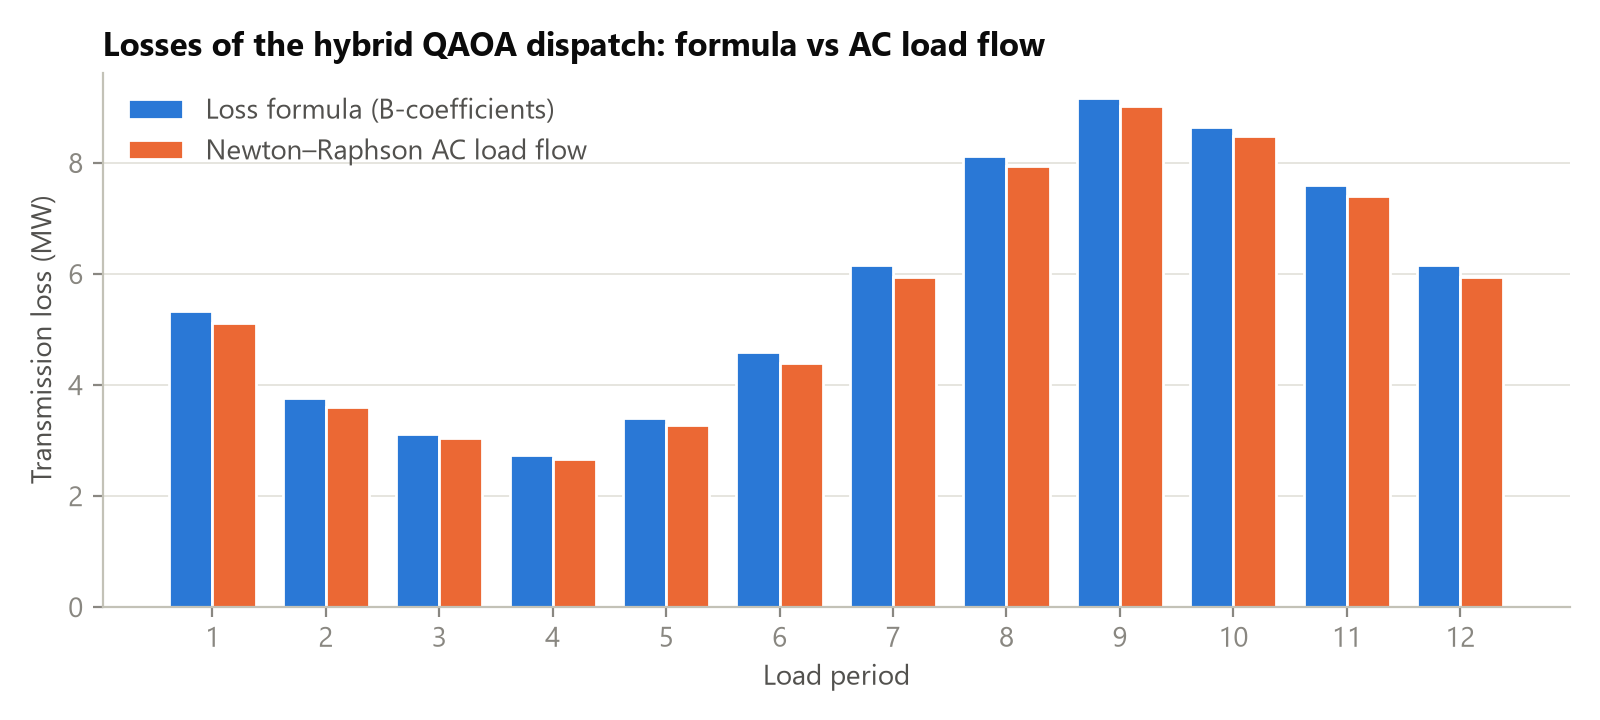
\includegraphics[width=0.9\textwidth]{losses}
\caption{Transmission losses of the hybrid QAOA dispatch: B-coefficient formula against Newton--Raphson.}
\label{fig:losses}
\end{figure}

\subsection{Voltages and reactive power}
All bus voltages stay between 1.009 and 1.070~pu, inside the 0.95--1.07~pu limits, and all generator reactive outputs stay inside their limits in every period.

\subsection{Line loading}
Figure~\ref{fig:lines} shows the loading of line T09 (bus 3 to bus 6), the most heavily loaded line in every period. It exceeds its 60~MVA continuous rating in periods 1 and 7--12, and its 75~MVA short-term rating in periods 8--11, reaching 145\,\% (87~MVA) at the 330~MW peak. The SLSQP optimum produces the same overloads in the same periods (142.7\,\% at the peak), so this is not caused by QAOA: it is a limitation of ELD itself, which ignores the network. G3 at bus 3 is the second-cheapest unit and feeds the load at bus 6 through the low-impedance line T09. Removing the overload requires security-constrained dispatch with line-flow limits, which is proposed as future work.

\begin{figure}[H]
\centering
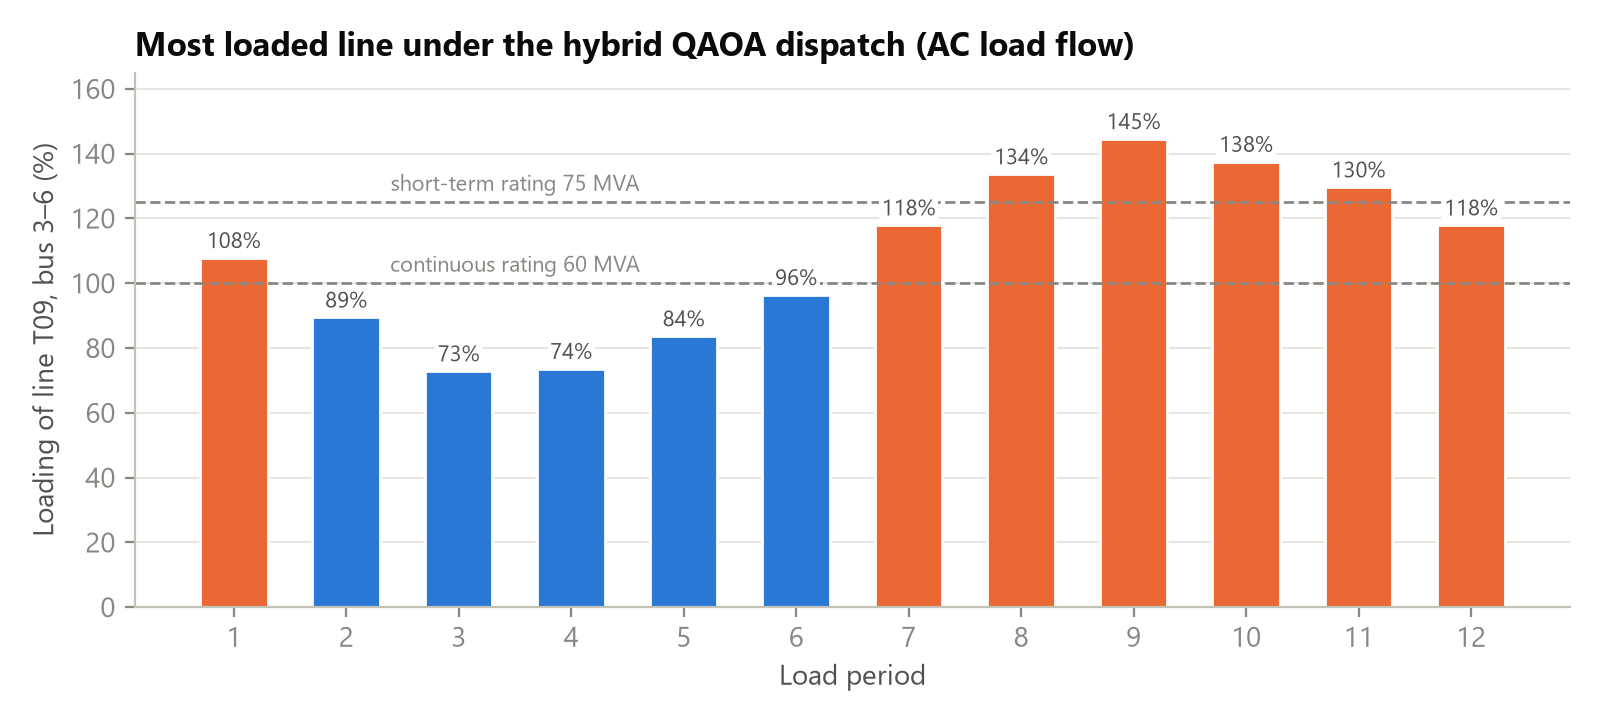
\includegraphics[width=0.9\textwidth]{line_loading}
\caption{Loading of line T09 under the hybrid QAOA dispatch (AC load flow).}
\label{fig:lines}
\end{figure}
